\documentclass{ctexart}
%导言区
\title{ctexart测试文档}
\author{向涛}
\date{\today}
\usepackage{booktabs}%三线表中\toprule \midrule \bottomrule的包以及\cmidrule{a-b}
\usepackage{amsmath,amssymb,amsfonts}%数学公式方面的包
\usepackage{array} %用于表格中整列的修饰,符号>{}r/c/l<{},{}中的内容是修饰关键词,可以是命令可以是符号等。并且还提供了表格中的上中下对其方式。
\usepackage{tabularx}%用于表格宽度分配均匀的宏包,\begin{tabularx}{14em}{XX},其中有两个必选参数,一个14是表格总宽度,XX表示表格中的内容格式。
\usepackage{multirow}%用于纵向合并单元格的宏包。
\usepackage{makecell}%拆分单元格,但无法画线。
\usepackage{graphicx}%插入图片的宏包。

\begin{document}
\maketitle   %显示引言区的内容

\section{引言}
这是一个关于 \LaTeX 的简单说明文档,主要讲述了关于一些特殊字符的命令,如何插入图片及表格,一些数学公式如何拼写并展示,最后是基于文档的排版,如页眉页脚的设计。

\section{特殊符号格式}
\subsection{常用的符号}
\# \$ \% \& \{ \} \_ \^{}  \~{} \textbackslash    % "# $ % & { } _ ^ ~ \"
%其中 \^ 和 \~ 两个命令需要一个参数,加一对花括号的写法相当于提供了空的参数

引号:``'',`'  ~~~  破折号:-,--,---  ~~~  省略号: $ \dots $ and $ \cdots $

还有很多符号此处不做说明。

\subsection{一些数学符号}
\subsubsection{巨算符}
\begin{gather}
   \sum ~~~~ \bigcup ~~~~ \bigvee ~~~~ \prod ~~~~ \bigcap ~~~~ \iint \\
  \idotsint~~~~\biguplus ~~~~ \bigotimes ~~~~ \oint ~~~~ \bigsqcup~~~~\iiint \\
   \bigwedge ~~~~  \coprod ~~~~ \int ~~~~ \bigodot ~~~~ \bigoplus ~~~~\iiiint
\end{gather}

\subsubsection{文本数学模型通用符号}
\begin{gather}
  \{ ~~~~ \} ~~~~ \$ ~~~~ \% ~~~~ \dag ~~~~ \S \\
  \copyright~~~~\dots ~~~~ \ddag ~~~~ \P ~~~~ \pounds
\end{gather}

\subsubsection{希腊字母}
\begin{gather}
\alpha~~~~\theta~~~~o~~~~\upsilon~~~~\beta~~~~\vartheta~~~~\pi~~~~\phi~~~~\gamma
\end{gather}

未完待续$\dots$
\section{表格}
\subsection{常用的三线表制作}


\subsection{一般表格制作}
\begin{tabular}{|*{2}{c|}m{6em}|m{4em}|}
\hline
1&2222&hello hi python & hello \\
\hline
\end{tabular}
我爱你中国

\[\dots\]

\begin{tabular}{>{\bfseries}rlc}
\hline
123&2222&3 \\
\hline
4&5&6 \\
\hline
\end{tabular}

\[\dots\]

\newcommand\txt
   {a b c d e f g h i}
\begin{tabular}{cp{2em}m{2em}b{2em}}
\hline
pos & \txt & \txt & \txt \\
\hline
\end{tabular}

\[\dots\]

\begin{tabularx}{18em}{|*{4}{>{\centering\arraybackslash}X|}}
\hline
A & B & C & D \\ \hline
a & b & c & d \\ \hline
\end{tabularx}

\[\dots\]

\begin{tabular}{|c|c|c|}
\hline
4 & 9 & 2 \\ \cline{2-3}
3 & 5 & 7 \\ \cline{1-1}
8 & 1 & 6 \\ \hline
\end{tabular}

\[\dots\]

\begin{tabular}{cccc}
\toprule
& \multicolumn{3}{c}{Numbers} \\
\cmidrule{2-4}
& 1 & 2 & 3 \\
\midrule
Alphabet & A & B & C \\
Roman
& I & II& III \\
\bottomrule
\end{tabular}

\[\dots\]

\begin{tabular}{|c|c|c|}
\hline
1 & 2 & Center \\ \hline
\multicolumn{2}{|c|}{3} &
\multicolumn{1}{r|}{Right} \\ \hline
4 & \multicolumn{2}{c|}{C} \\ \hline
\end{tabular}

\[\dots\]

\begin{tabular}{ccc}
\hline
\multirow{2}{*}{Item} &
\multicolumn{2}{c}{Value} \\
\cline{2-3}
& First & Second \\ \hline
A & 1& 2 \\ \hline
\end{tabular}

\[\dots\]

\begin{tabular}{|c|c|c|}
\hline
a & b & c \\ \hline
a & \multicolumn{1}{@{}c@{}|}
{\begin{tabular}{c|c}
e & f \\ \hline
e & f \\
\end{tabular}}
& c \\ \hline
a & b & c \\ \hline
\end{tabular}

\[\dots\]

\begin{tabular}{|c|c|}
\hline
a & \makecell{d1 \\ d2} \\
\hline
b & c \\
\hline
\end{tabular}

\[\dots\]

\renewcommand\arraystretch{2.8}
\begin{tabular}{|c|}
\hline
Really loose \\ \hline
tabular rows.\\ \hline
\end{tabular}

\[\dots\]

\begin{tabular}{c}
\hline
Head lines \\[6pt]
tabular lines \\
tabular lines \\ \hline
\end{tabular}

\section{如何插入图片}

\graphicspath{figure/}

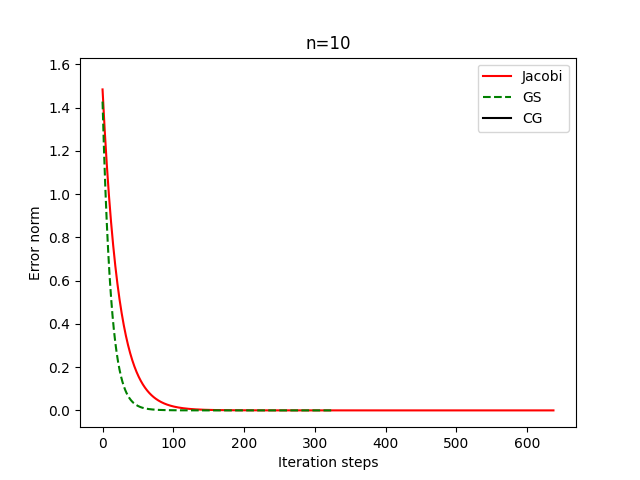
\includegraphics{Figure_10}


\includegraphics{lyf.jpg}

\begin{figure}
    \centering
    \begin{minipage}{8.5cm}
         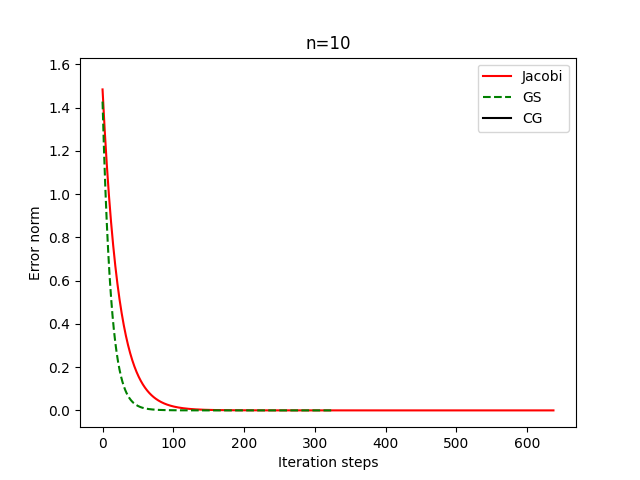
\includegraphics[scale= 0.5]{Figure_10}
    \end{minipage}
    \begin{minipage}{8.5cm}
         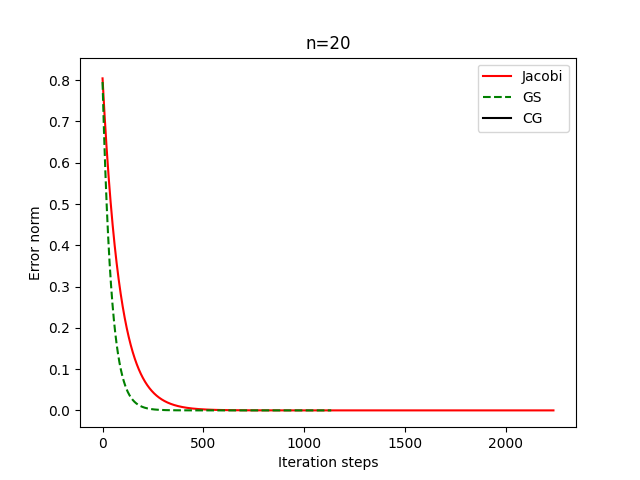
\includegraphics[scale= 0.5]{Figure_20}
    \end{minipage}
    
    \begin{minipage}{8.5cm}
         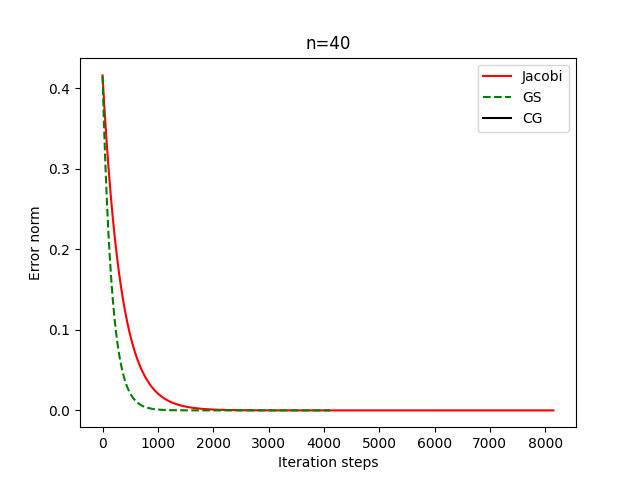
\includegraphics[scale= 0.5]{Figure_40}
    \end{minipage}
    \begin{minipage}{8.5cm}
         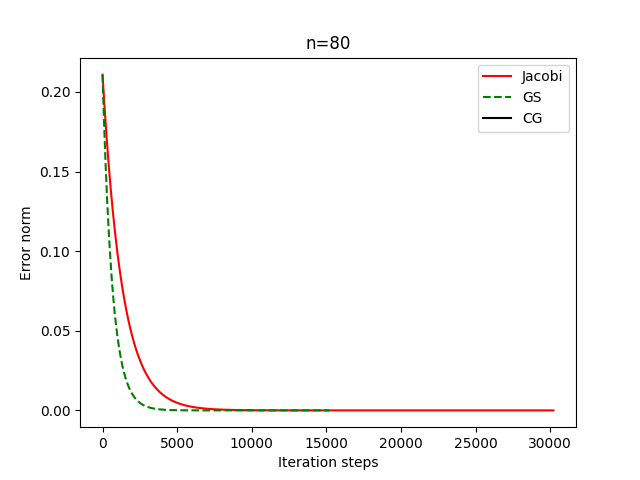
\includegraphics[scale= 0.5]{Figure_80}
    \end{minipage}
    \caption{迭代收敛误差曲线图}
\end{figure}  



\section{排版数学公式}

\section{页面排版设计}





\end{document}


     




